\chapter{Macros}

This program is almost fully automatable with macros. Macros
can be used to quickly analyze data. 
This program is capable of recording and running macros and
it is easy to write and modify macro files. 

\begin{SCfigure}[1][hbtp]
    \centering
    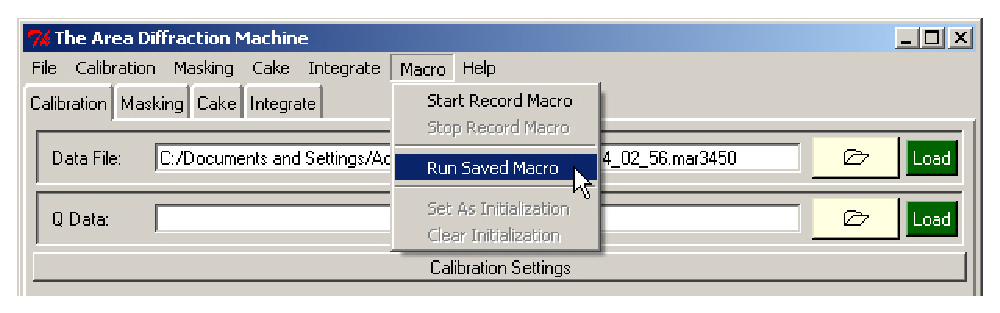
\includegraphics[scale=.75]{figures/macro.eps}
    \caption{The \gui{Macro} menu bar is used to
    record and run macros.}
    \label{macro_figure}
\end{SCfigure}

\section{Record and Run Macros}

The easiest way to create a macro is to record it by selecting 
the \gui{Start Record Macro} 
option in the \gui{Macro} menu 
bar shown in  figure~\ref{macro_figure}. 
After all of the desired steps are finished, 
the \gui{Stop Record Macro} option will save the macro to
a file. The \gui{Run Saved Macro} option in the \gui{Macro}
menu will run all the commands in a saved macro. 

\section{The Macro File Format}

A macro file is a list of commands, each on their own line, that tells the 
program what to do.
The syntax for macros is straightforward. Macro commands are the 
text corresponding to the part of the GUI that does 
the command. 
For example, the macro command \macroline{Get From Header} 
will get the calibration data from the header of the 
image.\footnote{Because of the ambiguity of some GUI items,
some macro command have different names. 
For example, the \gui{Number Of Chi} input shows up multiple
places in the program so the macro commands are instead
\macroline{Fit Number of Chi?}, \macroline{Integrate Number Of Chi?},
and \macroline{Cake Number Of Chi?}. When in doubt, 
section~\ref{macro_commands_table} has a list of all macro commands.}
Things get more interesting when the GUI item is more complicated
then a button. The \gui{Draw Q Data?} check box needs to know if it 
is selected or deselect. The macro command is
\begin{lstlisting}
Draw Q Data?
    Select
# Or, Deslect to not display them
\end{lstlisting}
Entering numbers is similar:
\begin{lstlisting}
beta:
    5.23
\end{lstlisting}
So are filenames:
\begin{lstlisting}
Save Caked Image
    C:/cake_output.jpg
\end{lstlisting}

\section{Looping Over Diffraction Data}
\label{LoopOverDiffractionData}

Diffraction data is loaded with the command
\begin{lstlisting}
Data File:
    C:/first.mar3450
\end{lstlisting}
Diffraction files in a list will be looped over and the same
analysis can be performed on all of them.
For example,
\begin{lstlisting}
Data File:
    C:/first.mar3450 C:/second.mar3450 
# ...
\end{lstlisting}
will run the subsequent macro lines on
the file \macroline{C:/first.mar3450} and
then on the file \macroline{C:/second.mar3450}.
The loop will end when one of three things happens: a subsequent line 
in the macro file is \macroline{END LOOP}, more diffraction data
is loaded using the \macroline{Data File:} command, or
the macro file ends. 

Directories can also be given. The program 
will (non-recursively) look for all diffraction
files in the directory and include them in the list. If the folder
\macroline{C:/data} contained the file \macroline{first.mar3450}
and \macroline{second.mar3450}, these files could
be looped over with the command
\begin{lstlisting}
Data File:
    C:/data/
# ...
\end{lstlisting}
Multiple folders and multiple files can be in the list.
They must be on the same line and separated by spaces.

\section{PATHNAME and FILENAME}

When a diffraction file is loaded by the macro,
any subsequent lines in the file will have
the string \macroline{PATHNAME} replaced with the
path of the current diffraction file and 
\macroline{FILENAME} replaced with the filename
of the current diffraction file.
For the file \macroline{C:/data/first.mar3450},
\macroline{PATHNAME} would be replaced by
\macroline{C:/data} and \macroline{PATHNAME} would
be replaced by \macroline{first}. A \macroline{.mar3450}
file could be reconstructed as 
\macroline{FILENAME/PATHNAME.mar3450}

While looping over multiple files, these commands can be used to
save things in useful places with useful names. It would be
easy, for example, to save intensity integrated data with the
macro:
\begin{lstlisting}
Save Integration Data
    FILENAME/PATHNAME\_int.dat
\end{lstlisting}
This would save the intensity data for
\macroline{C:/data/first.mar3450} as
\macroline{C:/data/first\_int.dat} and
the intensity data for \macroline{C:/data/second.mar3450} as
\macroline{C:/data/second\_int.dat}, etc. 

\section{Loading Multiple Images}

Multiple diffraction files can be loaded and their 
intensities added. The macro command to do this is
\macroline{Multiple Data Files} followed by a list of filenames
enclosed with [ and ] brackets. 
\macroline{C:/data/first.mar3450} and
\macroline{C:/data/second.mar3450} could be loaded at the
same time with the macro
\begin{lstlisting}
Multiple Data Files:
    [C:/data/first.mar3450 C:/data/second.mar3450]
# ...
\end{lstlisting}
All of the files that are added together must be in the same folder
so that that the \macroline{PATHNAME} syntax remains 
meaningful.
These sets of files can be looped over by putting
several of these bracketed lists on a line.
For example:
\begin{lstlisting}
Multiple Data Files:
    [C:/first.mar3450 C:/second.mar3450] [C:/third.mar3450 C:/fourth.mar3450]
# ...
\end{lstlisting}
will separately loop over \macroline{first.mar3450} 
and \macroline{second.mar3450} added together and then 
\macroline{third.mar3450} and \macroline{fourth.mar3450}
added together. Alternately,
all of the files that need to be analyzed can be grouped into 
subfolders. If each subfolder contains only files that should
be added together, the \macroline{Multiple Data Files} command
followed by the base folder will loop over each of the subfolders
and add all of the files in the subfolder together.
For example, suppose the folder \macroline{C:/data}
contained the sub folder \macroline{A} containing the files 
\macroline{first.mar3450} and \macroline{second.mar3450}
and suppose \macroline{C:/data} also contained the 
sub folder \macroline{B} containing the files
\macroline{third.mar3450} and \macroline{fourth.mar3450}.
The macro command
\begin{lstlisting}
Multiple Data Files:
    C:/data
# ...
\end{lstlisting}
would first load \macroline{first.mar3450} and 
\macroline{second.mar3450} and run the through loop.
It would then load \macroline{third.mar3450} and 
\macroline{fourth.mar3450} and run the through loop.
Multiple Lists of files and ] and multiple
folders containing subfolders can be put after
the \macroline{Multiple Data Files} line. They
must all be on the same line and separated by spaces.

Since the all the files added together must come
from the same folder, \macroline{PATHNAME} is
unambiguous. To avoid ambiguity, \macroline{FILENAME} 
is replaced by the string \macroline{MULTIPLE\_FILES}.

\section{FOLDERPATH and FOLDERNAME}

To facilitate writing macros that load and 
add together diffraction files in a loop, 
the program introduces the \macroline{FOLDERNAME}
and \macroline{FOLDERPATH} syntax.
\macroline{FOLDERNAME} will be replaced
by the name of the folder containing the current
diffraction file (or files). \macroline{FOLDERPATH} 
will be replaced by the path leading to the folder 
containing the file. A \macroline{mar3450}
file can be reconstructed as 
\macroline{FOLDERPATH/FOLDERNAME/FILENAME.mar3450}.
\macroline{FOLDERNAME} is useful because if multiple
files have been loaded at the same time, things can be saved
with the enclosing folders name. If multiple subfolders
are looped over, the output of the program for each set of 
files can be given a meaningful names if each of the subfolders
has a meaningful name.

\section{Setting Colors in a Macro}

There are several places in the program where a
color can be selected. Colors can be set from
inside a macro but the names of the colors is
a little confusing. The easiest way to figure out 
the syntax for setting a color is to record a macro,
set the color, and then copy and paste.

Technically, the program will accept 
any color which the tk GUI framework accepts. tk
will accept quite a few colors by their English name (such as 
\macroline{red}).\footnote{\url{http://wiki.tcl.tk/16166} 
contains a list of all the allowed color names.} 
Tk also accepts colors
by their RGB value. A color is written as \#
followed by the color's RGB value in hexadecimal.
Each red, green, and blue value ranges from 0 to 255 in
decimal and 00 to ff in hexadecimal. For example, \#ff0000 is red. 

\section{Little Tidbits}\label{Little Tidbits}
\begin{itemize}
    \item Macro commands are not case
    sensitive. The command \macroline{GeT fRoM hEaDeR} 
    is just as valid as 
    \macroline{Get From Header}. 
    \item White spaces at the beginning and end of a
    line are ignored. In the preceding examples, the
    spaces separating macro commands from input values
    was only there to increase readability. 
    \item New lines in a macro file are ignored.
    \item Comment lines beginning with \# 
    are ignored.
    \item The program will automatically move
    between tabs as it executes different commands 
    on different tabs. 
    \item Usually, macro commands will not be recorded
    when the macro item is selected through the menu bar. The
    only exceptions are items that can only be accessed
    that way.
\end{itemize}


\section{List of Macro Commands}\label{macro_commands_table}

\begin{center}

\setlongtables % keeps the width uniform across pages
\begin{longtable}{|p{4cm}|p{4cm}|p{7cm}|}
\caption{Macro Commands} \label{grid_mlmmh} \\

\hline \multicolumn{1}{|c|}{Command} & \multicolumn{1}{c|}{Followed By} & \multicolumn{1}{c|}{Effect} \\ \hline 
\endfirsthead

\multicolumn{3}{c}%
{{\bfseries \tablename\ \thetable{} -- continued from previous page}} \\

\hline \multicolumn{1}{|c|}{Command} & \multicolumn{1}{c|}{Followed By} & \multicolumn{1}{c|}{Effect} \\ \hline 
\endhead

\hline \multicolumn{3}{|r|}{{Continued on next page$\ldots$}} \\ \hline
\endfoot

\hline 
\endlastfoot
\multicolumn{3}{|c|}{Program State Commands}\\
\hline 
    \macrolinenoquotes{Work In eV}&None&Changes the state of 
        the program to work with the beam's energy.\\
    \macrolinenoquotes{Work in Lambda}&None&Changes the state of 
        the program so that the beam's wavelength.\\
    \macrolinenoquotes{Work in 2theta}&None&Changes the state of
        the program so that caking and intensity integration
        are done in $2\theta$ instead of $Q$.\\
    \macrolinenoquotes{Work in Q}&None&Changes the state of
        the program so that caking and intensity integration
        are done in $Q$ instead of $2\theta$.\\
    \hline
    \multicolumn{3}{|c|}{Calibration Commands} \\
    \hline
    \macrolinenoquotes{Data File:}&Files \& Directories&Opens
        a diffraction file and possibly loops over doing this.\\
    \macrolinenoquotes{Multiple Data Files"}&
        Files \& Directories&Loads several 
        several diffraction files and adding
        them together and possibly loops over doing this.\\
    %\macrolinenoquotes{Dark Current:}&Filename&Loads in the 
    %    Dark Current.\\
    \macrolinenoquotes{Q Data:}&Filename&Load in a $Q$ data file.\\
    \macrolinenoquotes{Standard Q}&$Q$ File&Loads in a
    standard $Q$ files. This command is followed by the name 
    in the standard $Q$ menu of one of the standards.\\
    \macrolinenoquotes{Get From Header:}&None&Gets the calibration 
        data from the image header.\\
    \macrolinenoquotes{Load From File:}&Filename&Loads a calibration 
        data file.\\
    \macrolinenoquotes{Previous Values}&None&Loads the previous
        calibration parameters.\\
    \macrolinenoquotes{Save To File}&Filename&Saves the calibration 
        data to a file.\\
    \macrolinenoquotes{xc:}&Number&Sets the $x$ center.\\
    \macrolinenoquotes{xc Fixed:} & \selectordeselect & Sets whether 
        or not to fix the $x$ center.\\
    \macrolinenoquotes{yc:}&Number&Set the $y$ center.\\
    \macrolinenoquotes{yc Fixed:}& \selectordeselect &Sets whether 
        or not to fix the $y$ center.\\
    \macrolinenoquotes{d:}&Number&Set the detector distance.\\
    \macrolinenoquotes{d Fixed:}& \selectordeselect &Sets whether 
        or not to fix the distance.\\
    \macrolinenoquotes{E:}&Number&Sets the energy. If the 
        program is in $\lambda$ mode, it will switch to $eV$ mode.\\
    \macrolinenoquotes{E Fixed:}& \selectordeselect &Sets whether 
        or not to fix the energy. If the program is in $\lambda$ mode,
        it will switch to $eV$ mode.\\
    \macrolinenoquotes{lambda:}&Number&Sets the wavelength. If
        the program is in $eV$ mode, it will switch to $\lambda$ mode.\\
    \macrolinenoquotes{lambda Fixed:}& \selectordeselect &Sets 
        whether or not to fix the wavelength. 
        If the program is in $eV$ mode, it will switch to $\lambda$ mode.\\
    \macrolinenoquotes{alpha:}&Number&Sets the $\alpha$ angle.\\
    \macrolinenoquotes{alpha Fixed:}& \selectordeselect &Sets whether 
        or not to fix the $\alpha$ angle.\\
    \macrolinenoquotes{beta:}&Number&Sets the $\beta$ angle.\\
    \macrolinenoquotes{beta Fixed:}& \selectordeselect &Sets whether 
        or not to fix the $\beta$ angle.\\
    \macrolinenoquotes{R:}&Number&Sets the rotation angle.\\
    \macrolinenoquotes{R Fixed:}& \selectordeselect &Sets whether 
        or not to fix the rotation angle.\\
    \macrolinenoquotes{pl}&Number&Sets the pixel length.\\
    \macrolinenoquotes{ph}&Number&Sets the pixel height.\\
    \macrolinenoquotes{Draw Q Lines?}&\selectordeselect&Sets whether 
        or not to draw constant $Q$ lines.\\
    \macrolinenoquotes{Draw Q Lines Color?}&color&Sets the color 
        of the constant $Q$ lines.\\
    \macrolinenoquotes{Draw dQ Lines?}&\selectordeselect&Sets wheter
        or not to draw constant $\Delta Q$ lines.\\
    \macrolinenoquotes{Draw dQ Lines Color?}&color&Sets the 
        color of the $\Delta Q$ lines.\\
    \macrolinenoquotes{Draw Peaks?}&\selectordeselect&
        Sets wheter or not to draw the fit peaks.\\
    \macrolinenoquotes{Draw Peaks Color?}&color&Sets the color of 
        the peaks.\\
    \macrolinenoquotes{Update}&None&Refreshes the diffraction image.\\
    \macrolinenoquotes{Save Calibration}&Filename&Saves the
        calibration parameters to a file.\\
    \macrolinenoquotes{Do Fit}&None&Fits the calibration parameters.\\
    \macrolinenoquotes{Make/Save Peak List}&Filename&Creates a peak 
        list and saves it to a file.\\
    \macrolinenoquotes{Use Old Peak List (if possible)?}&
        \selectordeselect&Sets whether or not to use previous peak lists
        when fitting.\\
    \macrolinenoquotes{Fit Number of Chi?}&Number&Sets the number of 
        $\chi$ slices around the diffraction image used
        when calibrating.\\
    \macrolinenoquotes{Stddev}&Number&The threshold for 
        allowing peaks.\\
    \hline    
    \multicolumn{3}{|c|}{Diffraction Display Commands} \\
    \hline
    \macrolinenoquotes{Diffraction Data Colormaps}&A colormap name&
        Sets the colormap used to display the diffraction data.\\
    \macrolinenoquotes{Diffraction Data Invert?}&\selectordeselect&
        Inverts the colormap used to display the diffraction data.\\
    \macrolinenoquotes{Diffraction Data Log Scale?}&\selectordeselect&
        Sets whether or not to use a log of the colormap.\\
    \macrolinenoquotes{Diffraction Data Low?}&Number from 0 to 1&Sets
        the percentage of maximum intensity that is mapped to the 
        lowest part of the colormap.\\
    \macrolinenoquotes{Diffraction Data Hi?}&Number from 0 to 1&Sets
        the percentage of maximum intensity that is mapped to the
        highest part of the colormap.\\
    \macrolinenoquotes{Save Diffraction Image}&Filename&Saves the 
        diffraction image to a file.\\
    \hline    
    \multicolumn{3}{|c|}{Masking Commands}\\
    \hline
    \macrolinenoquotes{Do Less Than Mask?}&\selectordeselect&
        Sets whether or not to apply a less than mask to the
        diffraction data.\\
    \macrolinenoquotes{(Pixels Can't Be) Less Than Mask:}&Number&
        Sets the less than mask.\\
    \macrolinenoquotes{Less Than Mask Color?}&color&Sets the
        color of the less than mask.\\
    \macrolinenoquotes{Do Greater Than Mask?}&\selectordeselect&
        Sets whether or not to apply a greater than mask to the
        diffraction data.\\
    \macrolinenoquotes{(Pixels Can't Be) Greater Than Mask:}&
        Number&Sets the greater than mask.\\
    \macrolinenoquotes{Greater Than Mask Color?}&color&Sets
        the color of the greater than mask.\\
    \macrolinenoquotes{Do Polygon Mask?}&\selectordeselect&
        Sets whether or not to use polygon masks.\\
    \macrolinenoquotes{Polygon Mask Color?}&color&Sets
        the color of the polygon masks.\\
    \macrolinenoquotes{Save Mask}&Filename&Saves all 
        polygon masks to a file.\\
    \macrolinenoquotes{Load Mask}&Filename&Loads all
        polygon masks from a file.\\
    \macrolinenoquotes{Clear Mask}&None&Removes ll
        polygon masks.\\
    \hline
    \multicolumn{3}{|c|}{Cake Commands}\\
    \hline
    \macrolinenoquotes{AutoCake}&None&Picks a 
        nice $Q$ and $\chi$ range and cakes.\\
    \macrolinenoquotes{Cake Q Lower?}&Number&Sets the lower $Q$ value 
        used when caking. If the program is in $2\theta$ mode, 
        it will switch to $Q$ mode.\\
    \macrolinenoquotes{Cake Q Upper?}&Number&Sets the upper $Q$ value 
        used when caking. If the program is in $2\theta$ mode, 
        it will switch to $Q$ mode.\\
    \macrolinenoquotes{Cake Number Of Q?}&Number&Sets the number of 
        $Q$ bins used when caking. If the program is 
        in $2\theta$ mode, it will switch to $Q$ mode.\\
    \macrolinenoquotes{Cake 2theta Lower?}&Number&Sets the lower 
        $2\theta$ value used when caking. If the program is in 
        $Q$ mode, it will switch to $2\theta$ mode.\\
    \macrolinenoquotes{Cake 2theta Upper?}&Number&Sets the upper
        $2\theta$ value used when caking. If the program is in 
        $Q$ mode, it will switch to $2\theta$ mode.\\
    \macrolinenoquotes{Cake Number Of 2theta?}&Number&Sets the
        number of $2\theta$ bins used when caking. If the program 
        is in $Q$ mode, it will switch to $2\theta$ mode.\\
    \macrolinenoquotes{Cake Chi Lower?}&Number&Sets the lower $\chi$ 
        value used when caking.\\
    \macrolinenoquotes{Cake Chi Upper?}&Number&Sets the upper $\chi$ 
        value used when caking.\\
    \macrolinenoquotes{Cake Number Of Chi?}&Number&Sets the number of 
        $\chi$ values used when caking.\\
    \macrolinenoquotes{Do Cake}&None&Performs the cake and displays 
        that caked data.\\
    \macrolinenoquotes{Last Cake}&None&Goes back to the previous 
        cake values.\\
    \macrolinenoquotes{Save Caked Image}&Filename&Saves the
        cake as a popular image format. The extension
        of the file tells the program what format
        to save the image as.\\
    \macrolinenoquotes{Save Caked Data}&Filename&Saves
        the cake to a file.\\
    \macrolinenoquotes{Cake Do Polarization Correction?}&
        \selectordeselect&Sets whether or not to apply
        a polarization correction when caking.\\
    \macrolinenoquotes{Cake P?}&Number from 0 to 1&Sets the 
        value of the polarization used when
        caking.\\
    \hline    
    \multicolumn{3}{|c|}{Cake Display Commands} \\
    \hline
    \macrolinenoquotes{Cake Data Colormaps:}&Colormap&
        Sets the colormap used to display the caked data.\\
    \macrolinenoquotes{Cake Data Invert?}&\selectordeselect&
        Sets whether or not to invert the colormap used to
        display the caked data.\\
    \macrolinenoquotes{Cake Data Log Scale?}&\selectordeselect&
        Sets whether or not to use a log scale of the colormap.\\
   \macrolinenoquotes{Cake Data Low?}&Number from 0 to 1&Sets
        the percentage of maximum intensity that is mapped to the 
        lowest part of the colormap.\\
    \macrolinenoquotes{Cake Data Hi?}&Number from 0 to 1&Sets
        the percentage of maximum intensity that is mapped to the
        highest part of the colormap.\\
    \hline    
    \multicolumn{3}{|c|}{Intensity Integration Commands}\\
    \hline
    \macrolinenoquotes{Integrate Q Lower?}&Number&Sets the lower
    $Q$ value used when integrating.
    If the program is in $2\theta$ mode, it will switch to $Q$ mode.\\
    \macrolinenoquotes{Integrate Q Upper?}&Number&Sets the upper
    $Q$ value used when integrating.
    If the program is in $2\theta$ mode, it will switch to $Q$ mode.\\
    \macrolinenoquotes{Integrate Number Of Q?}&Number&Sets the number of
    $Q$ bins used when integrating.
    If the program is in $2\theta$ mode, it will switch to $Q$ mode.\\
    \macrolinenoquotes{Integrate 2theta Lower?}&Number&Sets the lower
    $2\theta$ value used when integrating.
    If the program is in $Q$ mode, it will switch to $2\theta$ mode.\\
    \macrolinenoquotes{Integrate 2theta Upper?}&Number&Sets the upper
    $2\theta$ value used when integrating.
    If the program is in $Q$ mode, it will switch to $2\theta$ mode.\\
    \macrolinenoquotes{Integrate Number Of 2theta?}&Number&Sets the number of
    $2\theta$ bins used when integrating.
    If the program is in $Q$ mode, it will switch to $2\theta$ mode.\\
    \macrolinenoquotes{Integrate Chi Lower?}&Number&
    Sets the lower $\chi$ value used when integrating.\\
    \macrolinenoquotes{Integrate Chi Upper?}&Number&
    Sets the upper $\chi$ value used when integrating.\\
    \macrolinenoquotes{Integrate Number Of Chi?}&Number&
    Sets the number of $\chi$ bins used when integrating.\\
    \macrolinenoquotes{Integrate Q-I}&None&Performs a 
    $Q$ integration. If the program is in $2\theta$ mode, it 
    will switch to $Q$ mode.\\
    \macrolinenoquotes{AutoIntegrate Q-I}&None&Picks
    a good range of $Q$ values and does a $Q$ 
    integration. If the program is in $Q$ mode, 
    it will switch to $2\theta$ mode.\\
    \macrolinenoquotes{Integrate 2theta-I}&None&Performs
    a $2\theta$ integration. If the program is in $Q$ mode, 
    it will switch to $2\theta$ mode.\\
    \macrolinenoquotes{AutoIntegrate 2theta-I}&None&
    Picks a good range of $2\theta$ values and does
    a $2\theta$ integration. If the program is in $Q$ mode, 
    it will switch to $2\theta$ mode.\\
    \macrolinenoquotes{Integrate chi-I}&None&Performs
    a $\chi$ integration of the diffraction data.\\
    \macrolinenoquotes{AutoIntegrate chi-I}&None&Picks
    a good range of $\chi$ values and does
    a $\chi$ integration.\\
    \macrolinenoquotes{Save Integration Data}&Filename&
    Saves the integrated data to a file.\\
    \macrolinenoquotes{Constrain With Range On Right?}&
    \selectordeselect&Sets whether or not to 
    constrain the $Q$ or $2\theta$ integration 
    with the $\chi$ range.\\
    \macrolinenoquotes{Constrain With Range On Left?}&
    \selectordeselect&Sets whether or not to constraint
    the $\chi$ integration with the $Q$ or $2\theta$ range.\\
    \macrolinenoquotes{Integrate Do Polarization Correction?}&
    \selectordeselect&Sets whether or not to use a polarization
    correction when integrating.\\
    \macrolinenoquotes{Integrate P?}&Number form 0 to 1&Sets
    the polarization use when integrating.\\
    \macrolinenoquotes{Integration Data Log Scale?}&
    \selectordeselect&Sets whether or not to display
    integration data with a log scale.\\
\end{longtable}
\end{center}

\section{What Macros Can't Do}

\begin{itemize}
    \item There is no way with a macro to zoom into the diffraction
    data, the cake data, or the intensity integrated data
    \item polygon masks can not be drawn or individually removed
    from the program. Polygons can be loaded from a file with the
    \macroline{Load Mask} command and they can all be removed with the
    \macroline{Clear Mask} command.
    \item Diffraction data can only be loaded if it has a standard 
    file extension. 
\end{itemize}

